\documentclass{beamer}
\renewcommand\textbullet{\ensuremath{\bullet}}
\usetheme{Amsterdam}
\usepackage{lmodern}
\usepackage{tikz}
\usepackage{fontawesome}
\usepackage{verbatim}
\usepackage{adjustbox}
\usepackage{multicol}
\usetikzlibrary{decorations.text}
\usetikzlibrary{arrows,shapes,calc}
\usepackage{graphicx}
\graphicspath{ {./images/} }
\newcommand\blfootnote[1]{%
  \begingroup
  \renewcommand\thefootnote{}\footnote{\tiny  #1 }%
  \addtocounter{footnote}{-1}%
  \endgroup
}


\newcommand{\shrug}[1][]{%
\begin{tikzpicture}[baseline,x=0.8\ht\strutbox,y=0.8\ht\strutbox,line width=0.125ex,#1]
\def\arm{(-2.5,0.95) to (-2,0.95) (-1.9,1) to (-1.5,0) (-1.35,0) to (-0.8,0)};
\draw \arm;
\draw[xscale=-1] \arm;
\def\headpart{(0.6,0) arc[start angle=-40, end angle=40,x radius=0.6,y radius=0.8]};
\draw \headpart;
\draw[xscale=-1] \headpart;
\def\eye{(-0.075,0.15) .. controls (0.02,0) .. (0.075,-0.15)};
\draw[shift={(-0.3,0.8)}] \eye;
\draw[shift={(0,0.85)}] \eye;
% draw mouth
\draw (-0.1,0.2) to [out=15,in=-100] (0.4,0.95); 
\end{tikzpicture}}

\usepackage{listings}
\definecolor{mygreen}{rgb}{0,0.6,0}
\definecolor{mygray}{rgb}{0.5,0.5,0.5}
\definecolor{mymauve}{rgb}{0.58,0,0.82}

\lstset{ %
  %backgroundcolor=\color{white},   % choose the background color
  basicstyle=\tiny\ttfamily,        % size of fonts used for the code
  breaklines=true,                 % automatic line breaking only at whitespace
  captionpos=b,                    % sets the caption-position to bottom
  commentstyle=\color{mygray},    % comment style
  escapeinside={\%*}{*)},          % if you want to add LaTeX within your code
  keywordstyle=\color{mygreen},       % keyword style
  stringstyle=\color{blue},     % string literal style
}


\title{Monitoring ML applications in production}
\subtitle{An overview}

\author{Alexander Kim}

\date{Production AI Conference $\vert$ April 13th, 2019}

\subject{Production AI}

\begin{document}

\begin{frame}
 \titlepage
\end{frame}

\begin{frame}{Outline}
  \tableofcontents
\end{frame}


\section{Intro}

\begin{frame}{About me}
	Past:
  \begin{itemize}
  \item{B.Sc. \& M.Sc. in Physics @ (Moscow State University,  University of Alberta)}
  \item{Data Analysis \& Image Processing @ UrtheCast}
  \item{Data Science @ Splunk}
  \end{itemize}
	Currently:
  \begin{itemize}
  \item{Data Science @ [some private company \shrug]}
  \item{Organizer @ PyData Montreal}
  \end{itemize}
\end{frame}

\begin{frame}
	\begin{figure}%
	    \centering
	    \includegraphics[width=.45\linewidth]{urthecast_hrc.jpg}
	    \qquad
	    \includegraphics[width=.45\linewidth]{kiev_deimos.jpg}
	    \qquad
	    \blfootnote{source: urthecast.com}
	\end{figure}
\end{frame}

\begin{frame}
\centering
\includegraphics[width=.9\linewidth]{mltk_screenshot.png}
\blfootnote{source: splunk.com}
\end{frame}

%\begin{frame}
%\centering
%\includegraphics[width=.9\linewidth]{blur.jpg}
%\blfootnote{source: somewhere on the internet}
%\end{frame}

\begin{frame}{ML application life-cycle}{}
  \centering
  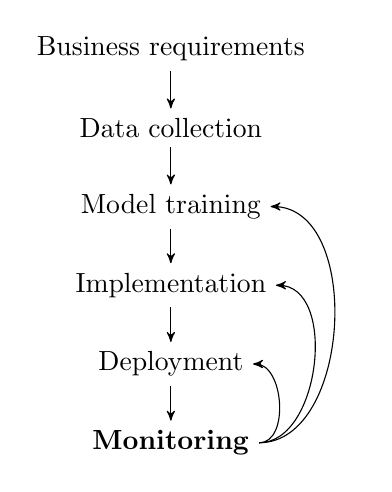
\begin{tikzpicture}[->,>=stealth',auto,node distance=1cm,main node/.style={}]

  \node[main node] (1) {Business requirements};
  \node[main node] (2) [below of=1] {Data collection};
  \node[main node] (3) [below of=2] {Model training};
  \node[main node] (4) [below of=3] {Implementation};
  \node[main node] (5) [below of=4] {Deployment};
  \node[main node] (6) [below of=5] {\textbf{Monitoring}};

  \path[every node/.style={}]
    (1) edge node [below] {} (2)
    (2) edge node [below] {} (3)
    (3) edge node [below] {} (4)
    (4) edge node [below] {} (5)
    (5) edge node [below] {} (6)
    (6) edge[in=0,out=0] node [auto] {} (3)
    (6) edge[in=0,out=0] node [auto] {} (4)
    (6) edge[in=0,out=0] node [auto] {} (5);
	\end{tikzpicture}
\end{frame}

\begin{frame}{Why monitor?}
	\centering
	No monitoring\\
	$\Big\Downarrow$\\
	End-user monitoring\\
	\pause
	$\Big\Downarrow$\\
	"Twitter monitoring"
	\begin{figure}
		\includegraphics[width=.4\textwidth]{twitter_screenshot_1.png}
	\end{figure}
	\pause
	
	\begin{tikzpicture}[overlay]
	\draw[line width=2mm,red] (0,4) circle (3);
	\draw[line width=2mm,red] ($(0,4)+(135:3)$)--($(0,4)+(-45:3)$);
	\end{tikzpicture}
\end{frame}

\begin{frame}{ML application layers}{What are we monitoring?}
	\begin{columns}[T] % align columns
		\begin{column}{.48\textwidth}
			\begin{itemize}
				\item {Infrastructure}
				\item {Code: performance and logic}
				\item {ML performance}
			\end{itemize}
		\end{column}
		
		\hfill
		
		\begin{column}{.48\textwidth}
			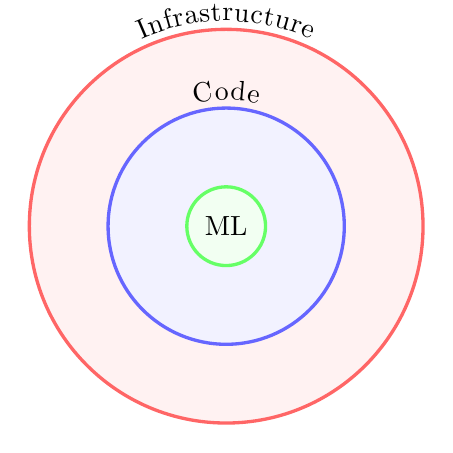
\begin{tikzpicture}
				\filldraw[color=red!60, fill=red!5, very thick, rotate=-90, postaction={decorate, decoration={text along path, raise=3pt, text align={align=center}, text={Infrastructure}, reverse path}}] (0,0) circle (2.5);
				\filldraw[color=blue!60, fill=blue!5, very thick, rotate=-90, postaction={decorate, decoration={text along path, raise=3pt, text align={align=center}, text={Code}, reverse path}}] (0,0) circle (1.5);
				\filldraw[color=green!60, fill=green!5, very thick] (0,0) circle (0.5);
				\draw (0,0) node {ML};
			\end{tikzpicture}
		\end{column}
	\end{columns}
\end{frame}

\section{Types of monitoring}

\subsection{Infrastructure monitoring}

\begin{frame}{Infrastructure monitoring}
  \begin{itemize}
  \item {Resource utilization \& Security: CPU, storage, network, etc.}
  \item {Tools: Zabbix, Nagios, Amazon CloudWatch, etc.}
  \end{itemize}
  	\begin{figure}%
	    \centering
	    \includegraphics[width=.45\linewidth]{zabbix_dashboard.png}
	    \qquad
	    \includegraphics[width=.45\linewidth]{nagios_dashboard.png}
	    \qquad
	    \blfootnote{source: zabbix.com, nagios.com}
	\end{figure}
\end{frame}

\subsection{Code monitoring}

\begin{frame}{Code monitoring}
	\begin{itemize}
		\item{Instrumentation \& metrics: \textbf{statsd, prometheus}, etc.}
  		\item{Event logging \& tracing: \textbf{logstash, splunk}, etc.}
  		
	\end{itemize}
	% Difference: metrics VS logging and tracing
	% High-level view vs Individual events
\end{frame}

\begin{frame}{Instrumentation \& metrics: Statsd}
  	\begin{itemize}
  		\item{API client \rightarrow UDP protocol \rightarrow Daemon \rightarrow Collection backend}
  		\item{Lightweight and simple, non-blocking, dimensional data model} % no logical hierarchy
  		\item{Metric types: counters, timers, gauges, sets}
  		\item{External data storage} % graphite, influxdb, datadog
	\end{itemize}
\end{frame}

\begin{frame}{Instrumentation \& metrics: Statsd}
	\centering
   	\includegraphics[width=.7\linewidth]{statsd_data_flow.png}
   	\blfootnote{source: https://www.youtube.com/watch?v=NydIHi8Y224}
\end{frame}


\begin{frame}{Instrumentation \& metrics: Prometheus}
	\begin{itemize}
		\item{Statsd-like functionality and more}
		\item{Built-in TSDB and dashboard, local storage*} % scalability limitations by design (clustering is hard)
		\item{PromQL, Alerting}
	\end{itemize}
\end{frame}

\begin{frame}{Instrumentation \& metrics: Prometheus}
	\centering
	\includegraphics[width=.9\linewidth]{prometheus_arch.png}
	\blfootnote{source: https://www.youtube.com/watch?v=PDxcEzu62jk}
\end{frame}


\begin{frame}[fragile]{Instrumentation \& metrics: Statsd vs Prometheus}
	\begin{block}{Statsd}
	\begin{lstlisting}[language=python]
...# other imports here
import statsd
c = statsd.StatsClient("my_host_name", 8125)
...# application code here
c.incr('http_requests_total.home.400')
	\end{lstlisting}
	\end{block}
	
	\begin{block}{Prometheus}
	\begin{lstlisting}[language=python]
...# other imports here
from prometheus_client import Counter
c = Counter('http_requests_total', 'Total HTTP Requests (count)', ['method', 'endpoint', 'status_code'])
...# application code here
c.labels(method='GET', endpoint="/home", status_code=400).inc()
	\end{lstlisting}
	\end{block}
\end{frame}


\begin{frame}[fragile]{Instrumentation \& metrics: Statsd vs Prometheus}
	\begin{itemize}
		\item{Simplicity and low overhead \rightarrow Statsd}
		\item{Large number of service instances \rightarrow Prometheus} % microservices, containers
		\item{from Statsd to Prometheus: \url{https://github.com/prometheus/statsd_exporter}}
	\end{itemize}
\end{frame}


\begin{frame}{Instrumentation \& metrics: Visualization}
	\centering
	\includegraphics[width=.9\linewidth]{grafana_screenshot.png}
	\blfootnote{source: https://azure.microsoft.com/en-us/blog/monitor-azure-services-and-applications-using-grafana}
\end{frame}


\begin{frame}{Event logging \& tracing}{Elastic Stack}
% inputs, filters, outputs; beats, grok patterns; x-pack
	\begin{itemize}
		\item{Logstash \& Beats}
		\item{Elasticsearch}
  		\item{Kibana}
  		\item{Elastic Stack Features (X-Pack)}
	\end{itemize}
	\pause
	\includegraphics[width=.9\linewidth]{logstash_example.png}
	\blfootnote{source: https://medium.com/oneclicklabs-io}
\end{frame}


\begin{frame}{Elastic Stack}{Logstash}
	\begin{block}{Logstash config}
	\centering
		\includegraphics[width=0.4\linewidth]{logstash_config.png}
	\end{block}
\end{frame}


\begin{frame}{Elastic Stack}{Kibana}
	\begin{block}{Kibana Dashboard}
		\centering
		\includegraphics[width=0.8\linewidth]{kibana_screenshot.png}
	\end{block}
	\blfootnote{source: https://www.elastic.co}
\end{frame}

\begin{frame}{Elastic Stack}{X-Pack}
	\begin{block}{Elastic Stack Features (X-Pack)}
		\centering
		\includegraphics[width=0.8\linewidth]{kibana_anomaly_detection.jpg}
	\end{block}
	\blfootnote{source: https://www.elastic.co}
\end{frame}


\begin{frame}{Elastic Stack vs Splunk, Sumo Logic, etc.}
	\begin{itemize}
		\item{Open-source vs proprietary}
		\item{Customization vs off-the-shelf features}
  		\item{Pay developers vs pay company}
	\end{itemize}
	\begin{multicols}{2}
        \begin{figure}[ht!]
            \includegraphics[width=.2\textwidth]{sumo_logic_logo}\hfill
            \includegraphics[width=.2\textwidth]{splunk_logo}\hfill
            \includegraphics[width=.2\textwidth]{datadog_logo}\hfill
            \includegraphics[width=.2\textwidth]{new_relic_logo}
        \end{figure}
    \end{multicols}
\end{frame}


\subsection{Monitoring ML components}

\begin{frame}{ML monitoring}
	\begin{itemize}
		% credit card fraud, logistics/shipping 
		\item{Comparison with ground truth}
  		\item{Human-in-the-loop ML}
  		\item{Model decay}
	\end{itemize}
\end{frame}


\begin{frame}{Human-in-the-loop ML}
	\begin{itemize}
		\item{Frees engineers from edge cases} % high loss, high uncertainty, low pred probability. Requires a team of human supervisors/experts.
		\item{Might be critical in some industries or mandated by law}
		\item{Content moderation teams, medical professionals, stylists, etc.}
		% stitchfix, netflix
	\end{itemize}
\end{frame}


\begin{frame}{Human-in-the-loop ML}
	\begin{figure}
		\centering
		\includegraphics[width=0.8\linewidth]{stitchfix_flow.png}
	\end{figure}
	% cernsoring, "survivorship" bias
	\blfootnote{source: youtube.com/watch?v=\_m8YOfnv-sg}
\end{frame}


\begin{frame}{Model decay}
	\begin{itemize}
		\item{Distributions change over time:}
		\begin{itemize}
			\item{Macroeconomic factors} % e.g. credit rating 
			\item{Data sources/integration} % e.g. time units, DST
			\item{Internal changes (policy, strategy, UX, etc.)} 
		\end{itemize}
		\item{Statistical tests} 
		% differences between distributions
		% average is not a good metric
	\end{itemize}
\end{frame}


\begin{frame}{Statistical tests: feature X}{training and observed samples}
	\begin{figure}
		\centering
		\includegraphics[width=0.7\linewidth]{two_dist.png}
	\end{figure}
\end{frame}


\begin{frame}{Statistical tests: feature X}{training and observed samples}
	\begin{figure}
		\centering
		\includegraphics[width=0.8\linewidth]{two_dist_code.png}
	\end{figure}
\end{frame}


\begin{frame}{Population Stability Index (PSI)}
	$$PSI=\sum((X_{train}\% - X_{observed}\%)*ln(\frac{X_{train}\%}{X_{observed}\%}))$$
	\begin{table}[ht]
	\centering
	\begin{adjustbox}{width=\textwidth}
		\begin{tabular}{|l|l|}
		\hline
		\textbf{PSI Value} & \textbf{Recommendation} \\
		\hline
		less than 0.1 & No action required \\
		\hline
		between 0.1 and 0.25 & Need to investigate and understand the changes \\
		\hline
		greater than 0.25 & Feature X is no longer a good feature for this model \\
		\hline
		\end{tabular}
	\end{adjustbox}
	\end{table}

	% equal sized buckets or quantiles
	% downside: can not be computed if a bucket has 0 items in it
\end{frame}

\begin{frame}{Population Stability Index (PSI)}
	\begin{figure}
		\centering
		\includegraphics[width=0.8\linewidth]{psi_calc.png}
	\end{figure}
\end{frame}


\begin{frame}{Kolmogorov–Smirnov test}
	$$D=max(abs(CDF_{training} - CDF_{observed}))$$
	\begin{figure}
		\centering
		\includegraphics[width=0.6\linewidth]{two_dist_cdf.png}
	\end{figure}
\end{frame}


\begin{frame}{KS test}{Scenario: mean of feature X decreases over time}
	\begin{figure}
		\centering
		\includegraphics[width=0.7\linewidth]{ks_ex_1.png}
	\end{figure}
\end{frame}

\begin{frame}{KS test}{Scenario: mean of feature X decreases over time}
	\begin{figure}
		\centering
		\includegraphics[width=0.7\linewidth]{ks_ex_2.png}
	\end{figure}
\end{frame}

\begin{frame}{KS test}{Scenario: mean of feature X decreases over time}
	\begin{figure}
		\centering
		\includegraphics[width=0.7\linewidth]{ks_ex_3.png}
	\end{figure}
\end{frame}


\begin{frame}{Other ways to detect change}
	\begin{itemize}
		\item{Loss function values vs time}
		\item{Model uncertainty vs time}
	\end{itemize}
\end{frame}



% Placing a * after \section means it will not show in the
% outline or table of contents.
\section{Summary}

\begin{frame}{Summary}
  \begin{itemize}
  \item
    Production is an opportunity for learning
  \item
  	Good monitoring = automated monitoring
  \item
    Monitoring will evolve along-side your application: start simple
  \item
    Monitoring in phases e.g.:
    \begin{enumerate}
    \item
      File logging + simple metrics + dashboards
    \item
      + logging to data store systems + threshold-based alerting
    \item 
      + ML-based monitoring and alerting
    \item
      + model decay monitoring
    \end{enumerate}
  \end{itemize}
\end{frame}

\begin{frame}{Additional Resources}
	\begin{itemize}
	\item{Sculley, David, et al. "Hidden technical debt in machine learning systems." Advances in neural information processing systems. 2015.}
	\item{Breck, Eric, et al. "What’s your ML Test Score? A rubric for ML production systems." (2016).}
	\item{Polyzotis, Neoklis, et al. "Data management challenges in production machine learning." Proceedings of the 2017 ACM International Conference on Management of Data. ACM, 2017.}
	\end{itemize}
\end{frame}

{
\usebackgroundtemplate{\includegraphics[width=\paperwidth]{niagra_falls.jpg}}%
\begin{frame}{Thank you!}
	\begin{minipage}{0.7\textwidth}
	\begin{itemize}
		\item[]{alexkimxyz @ \href{https://github.com/alexkimxyz}{\faGithub} $\vert$ \href{https://www.linkedin.com/in/alexkimxyz/}{\faLinkedin} $\vert$ \href{https://twitter.com/alexkimxyz}{\faTwitter}}
		\item[]{alexander.kim@ualberta.ca}
		\item[]{}
		\item[]{}
		\item[]{}
  	\end{itemize}
  	\end{minipage}
\end{frame}
}

\end{document}


